\Chapter{Üzleti folyamatok és modellezésük}

%általános áttekintést kellene adjon arról, hogy mik azok az üzleti folyamatok, hogyan szokták modellezni őket, milyen matematikai modellek vannak, egyáltalán miért lényeges, milyen szoftveres eszközök vannak.

Dolgozatom első tartalmi fejezetének alapjául a(z) \cite{xflower} forrás blogbejegyzéseit használtam, ezeket dolgoztam fel és egészítettem ki önálló gondolatokkal.

\Section{Mik azok az üzleti folyamatok?}

Elsőként nézzük meg, mit nevezhetünk egy folyamatnak. A folyamat szó más-más jelentéssel bír annak függvényében, hogy hol használjuk: például mást jelent a hétköznapi életben, mint az informatikában. A mi esetünkben a folyamat előre meghatározott vagy tetszőleges sorrendben elvégezhető tevékenységek kapcsolatrendszerét jelent.

Tehát gyakorlatilag a folyamat olyan tevékenységek halmaza, amelyek egymással kölcsönhatásba lépnek egy adott cél elérése érdekében. Ezt a jelentését használhatjuk az üzleti folyamatokra is, hiszen ha egy üzleti célt tűzünk ki magunk elé, akkor annak megvalósulása is több tevékenység egymásutániságából, több lépésből fog adódni. Ezeket a lépéseket együttesen nevezzük \textit{üzleti folyamat}nak.

Alapvetően kétféle megközelítése van a lépések végrehajtásának sorrendjének:

\begin{itemize}
\item Tevékenységek tetszőleges sorrendben elvégezhetőek.
\item Csak egymás utáni, meghatározott sorrendben követhetik egymást.
\end{itemize}

Az üzleti folyamatok minden vállalat életében napi szinten jelen vannak és egy áttekinthető láncolatot alkotnak a termék előállításához szükséges nyersanyagok beszerzésétől kezdve a munkafolyamatokon keresztül egészen a piacra kerülésig, és a piacon való sikeres vagy sikertelen szereplésig.

Üzleti folyamatokról általában akkor beszélünk, ha egy adott vállalat termékét, szolgáltatását, vagy menedzsmentjét akarjuk elhelyezni a gazdasági életben. Belátható, hogy a termék minősége és mennyisége összefügg a gyártó menedzsmentjének arculatával, piaci ismertségével, és a termék iránti kereslet erejével. Ezeket az összefüggéseket jeleníti meg egy vállalat reklám, PR, és marketing tevékenysége, melyről később lesz szó. Közismert példa, hogy az MGM stúdió világ viszonylatban piacvezető termékeket (filmeket) állít elő, de sikere a filmgyártás és forgalmazás költségeinek (reklám, PR, marketing) mértéke azonos vagy a forgalmazás irányában nagyobb mértékű.

Hogy érthetőbb legyen mit is jelent a gyakorlatban az üzleti folyamat, nézzük rá egy egyszerű példát:

Adott egy startup (vagy magyarosabban \textit{korai fázisú vállalkozás} FORRÁS: widipedia), ahol szükségessé válik bizonyos irodaszerek beszerzése. Magát a beszerzés menetét egy kizárólag kötött sorrendben elvégezhető folyamat fogja leírni. Nézzük a folyamat lépéseit:

\begin{enumerate}
\item Első lépésben konkrétan meghatározzák, hogy melyek azok az eszközök, amelyekre szükség van, és miből hány darab szükségeltetik. Ezeknek az összeírása az első feladat.

\item Miután összegyűjtötték a megrendelendő tárgyakat, meg kell vizsgálniuk, hogy a vállalkozás mekkora anyagi kerettel rendelkezik, és ebből mennyit tudnak a megrendelésre költeni. Ha rendelkeznek megfelelő pénzösszeggel, akkor minden rendben van, tovább lehet lépni. Ha viszont nem, akkor valamilyen szempont alapján ki kell húzni a listáról bizonyos termékeket (például a legszükségtelenebbeket). Ez utóbbi termékek megrendelése vagy elvetése a következő lépéstől is függ.

\item Ha már rendelkezésükre áll a lista és a pénzügyi fedezet, utána kell nézniük, hogy az adott eszközök hol szerezhetőek be a legalacsonyabb áron (ehhez segítséget tud nyújtani például a \url{https://www.arukereso.hu/} oldal, ami ár szerinti növekvő sorrendben kilistázza, hogy egy adott termék mely online webáruházakban és milyen áron érhetők el). Természetesen nem csak az alacsony ár, hanem más szempont is szóba jöhet (például a garancia időtartalma az adott termékre, a kiszállítás díja, stb.).

Ennél a lépésnél derül ki, hogy pontosan mennyi összeget kell a meglévő pénzügyi keretből az új eszközök megrendelésére fordítani. Lehetséges, hogy marad még pénz egy korábban az anyagi keret szűkösségére való hivatkozás miatt lehúzott termék megvásárlására.

\item Mindezek után elindulhat a megrendelés folyamata. Ez többféleképpen is történhet:

\begin{itemize}
\item Az eszközöket online rendeljük meg. Ennek előnye, hogy egyszerre több helyen is megfigyelhetjük a termékeket, utána járhatunk az azokat árusító weboldalak hitelességének, megbízhatóságának, véleményeket olvashatunk róla, és nem kell személyesen megjelennünk az adott áruházban. Hátránya, hogy időbe telik a termékek kiszállítása, és adott esetben számolnunk kell a szállítási költséggel is. Ez utóbbinak mértéke áruházanként eltérő. Ugyanakkor ma már léteznek olyan webáruházak is, ahol a megrendelt terméket személyesen is át lehet venni egy előre meghatározott üzlethelységben, így azokhoz gyorsabban juthatunk hozzá, viszont ebben az esetben a megrendelőre hárul a szállítási költség.

\item Megtehetjük, hogy nem rendeljük meg előzetesen a termékeket, hanem azok beszerzésére személyesen megyünk be az áruházakba. Ezt akkor célszerű alkalmaznunk, mikor egy nagyobb áruházat fogunk meglátogatni, ahol nagy eséllyel az összes termék rendelkezésünkre fog állni, így azokat egy helyről azonnal meg is tudjuk venni, és elvinni. Nagy előny ebben az esetben (szemben az online rendeléssel), hogy ki is tudjuk próbálni az adott termékeket, hogy hogyan működnek, van-e valamilyen hibájuk.
\end{itemize}

\item Ezek után, hogy a megrendelt termékek eljutottak az irodába, utolsó lépésként már csak szét kell osztani azokat aszerint, hogy mely terméket ki igényelte.

Ezzel a végére is értünk egy egyszerűbb üzleti folyamatnak.
\end{enumerate}

Azért ezt a fenti példát hoztam szemléltetésként, mert ez valamilyen formában minden vállalkozásnál jelen van. Ha jobban belegondolunk, láthatjuk, hogy gyakorlatilag szinte minden tevékenységet (így adott termék vagy termékek beszerzését is) folyamatban végzünk. Fontos megjegyezni, hogy ennél a példánál, és az ehhez hasonlóknál a lépéseket csak adott sorrendben hajtódhatnak végre. Például nem vihetünk el egy terméket az áruházból úgy, hogy csak majd később fizetünk érte.

%A szakirodalomban a fentieken kívül az alábbi üzleti folyamatokat találjuk meg:

%Az üzleti folyamatok meghatározására jelentős mértékű szakirodalom áll rendelkezésünkre.
%felsorolás
%Ezek közül a dolgozat témájához XY definícióját érzem a legpontosabbnak. Ennek mentén próbálom kifejteni téziseimet az üzleti folyamatokról és modellezésükről.

%Az üzleti folyamat alatt adott tevékenységek bizonyos szempont szerinti összekötését, avagy előre megadott sorrend szerinti egymásutániságát értjük. 

%Az üzleti folyamatok (\textit{Business processes}, BP) alatt azokat a folyamatokat értjük, amelyek biztosíthatják, hogy a személyek következetesen adják meg az adatokat, és mindig ugyanazokat a lépéseket kövessék minden alkalommal, amikor egy ügyféllel dolgoznak az üzleti folyamatok létrehozásán.

%A folyamat – esetünkben üzleti folyamat – bizonyos tevékenységek láncát, avagy adott sorrend szerint egymásutániságát jelenti. Magyarán szólva, ha kitűzünk egy üzleti jellegű célt, annak megvalósításához utunk több lépésen keresztül fog vezetni. Ezen lépések együttesen jelentik az üzleti folyamatot, melyben bizonyos tevékenységek tetszőleges sorrendben végezhetőek el, míg mások kizárólag egymás után következhetnek.

%Üzleti folyamatok: termék/szolgáltatás kiválasztása, fizetése vagy használata

\begin{figure}[h]
\centering
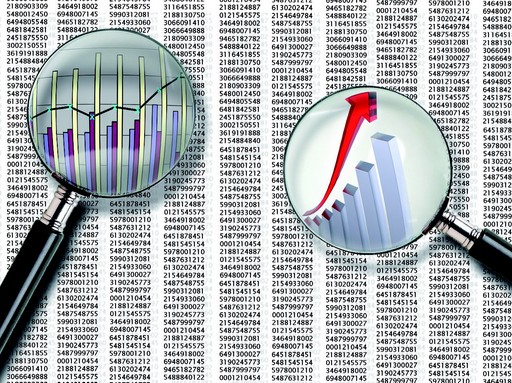
\includegraphics[scale=0.5]{images/uzleti_intelligencia.png}
\caption{Üzleti intelligencia (forrás: piacesprofit.hu)}
\label{fig:uzlint}
\end{figure}

%\SubSection{Miért lényegesek?}

%Meghatározzák a vállalatok mindennapjait.

\Section{Üzleti folyamatok modellezése}

Az előző részben olvashattuk, hogy nagyon sok mindent folyamatban végzünk. Akár egy legegyszerűbb hétköznapi tevékenységet is. Egy vállalat esetében pedig az ilyen tevékenységekből jóval több van, melyek lényeges szerepet játszanak annak működésében. Emiatt fontos az, hogy a vállalat bizonyos folyamatai rögzítésre kerüljenek. Ezért van szükség a folyamatok \textit{modellezésére}. Ennek egy egyszerű, átlátható formája a folyamatábra használata.

\SubSection{Modellezés folyamatábrával}

%https://xflower.hu/blog/az-uzleti-folyamatokrol-bovebben-vi-a-folyamatabra-alapjai esetleg még innen átvett dolgokkal kiegészíthető

A folyamatábra gyakorlatilag egy olyan eszköz, amely segítségével grafikusan ábrázolhatóak a tevékenységek, folyamatok. A különböző folyamatokat különböző szimbólumokkal jelölhetjük rajta, közöttük sorrendiséget állíthatunk fel meghatározva ezáltal azt, hogy időben melyik esemény melyik után vagy előtt következik be. Hogy érthetőbb legyen, miről is van szó, \aref{fig:folyamata} ábra egy nagyon egyszerű folyamatábrát szemléltet, amin a szakdolgozatom készítésének legfőbb lépései helyezkednek el.

\begin{figure}[h]
\centering
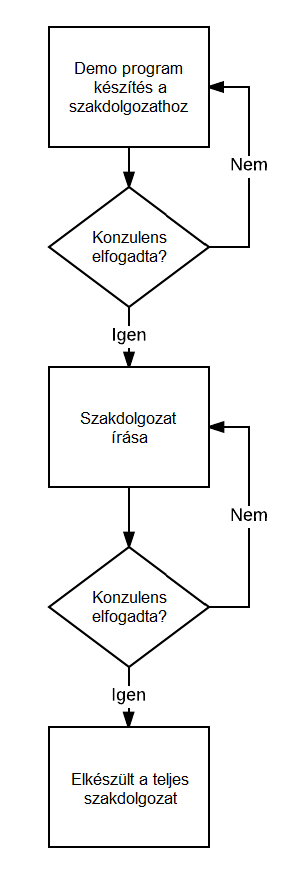
\includegraphics[scale=0.7]{images/folyamatabra.png}
\caption{Egy egyszerű folyamatábra}
\label{fig:folyamata}
\end{figure}

\newpage %Egybe legyen, aminek egybe kell lennie

A fent látható folyamatábra egyszerűségét az is adja, hogy nem teljes. Nincsen kiindulópontja sem végpontja. Olyan, mintha egy nagyobb folyamatból csak néhány tevékenységet ábrázolnánk. Ahhoz, hogy teljes legyen a folyamatábra, szükség van kezdő- és végállapotra.

Nézzük tehát, hogy mitől lesz teljes egy folyamatábra, illetve hogy általánosságban milyen részeket tartalmaz. Az alábbi (leggyakoribb, szinte minden folyamatábrán megtalálható) szimbólumok a következő jelentéssel bírnak:

\begin{itemize}
\item \textit{Téglalap} jelöli a tevékenységet. Ebből van a legtöbb a folyamatábrán, hiszen ezek szemléltetik magát a folyamatot, az események egymás utáni történését.
\item \textit{Rombusz} alak jelenti az átjárókat. Ezek útválasztóként funkcionálnak azáltal, hogy egy feltételt szabnak meg, melynek kiértékelésétől függ, hogy melyik tevékenység fog következni. Általában két másik tevékenység követi, amelyek közül az lesz a soron következő, amelyikre az útválasztó kiértékelése a megfelelő (igaz vagy hamis) értéket adja.
\item \textit{Üres fehér kör vékony fekete körívvel} fejezi ki a "START" állapotot \textit{(kezdőállapot)}. Itt kezdődik el a reprezentált folyamat. Legalább egy "START" szimbólumot tartalmaznia kell minden folyamatábrának.
\item A folyamat befejezését az \textit{üres fehér kör vastag fekete körívvel} jelöli. Ezt "END" állapotnak \textit{(végállapotnak)} is szokták nevezni. Ebből is legalább egynek lennie kell, hiszen ahogy elkezdődik egy folyamat, úgy az be is fejeződik egy bizonyos idő után. Előfordul olyan folyamatábra, ami több végállapotot tartalmaz, mint kezdőállapotot. Ez nem hiba, hiszen a való életben is gyakran fejeződik be egy elkezdett folyamat többféleképpen.
\item A különböző folyamatokat nyilak kötik össze, melyeket \textit{szekvenciafolyam}nak neveznek. Fontos, hogy ezek nem lehetnek csak vonalak nyíl nélkül, hiszen egyértelműen meg kell határozniuk, hogy melyik tevékenységből melyik másik következik.
\end{itemize}

Példaként tekintsük \aref{fig:uresfolyamat} ábrát, ami egy teljes folyamatábrát mutat, mely a fent említett szimbólumok közül mindegyikből tartalmaz legalább egyet (beleértve a kezdő- és végállapotokat is).

\begin{figure}[h]
\centering
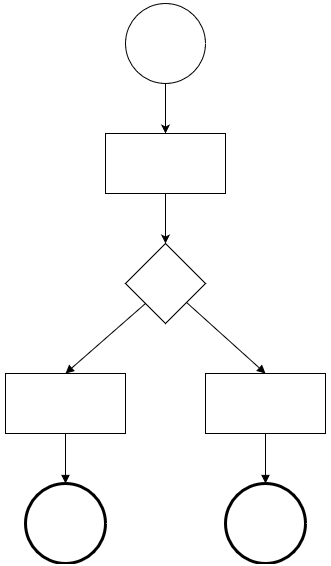
\includegraphics[scale=0.8]{images/uresfolyamat.png}
\caption{Egy üres, de teljes folyamatábra (Forrás: draw.io)}
\label{fig:uresfolyamat}
\end{figure}

Természetesen léteznek ennél sokkal összetettebb, többféle szimbólumot tartalmazó folyamatábrák is, azonban már egy ekkora ábrán is meg lehet jeleníteni egyszerűbb üzleti folyamatokat.

\Section{Egy folyamatokat szemléltető szoftveres eszköz}

\SubSection{Draw.io}

Folyamatok ábrázolására már nagyon sok kész program létezik. Például \aref{fig:uresfolyamat} ábrát is egy ilyen folyamatábrázoló szoftver segítségével készítettem el, melynek neve \textit{Draw.io}\cite{drawio}. A Draw.io a legismertebb és legsokoldalúbb ingyenes folyamatábrázoló alkalmazás. Az alkalmazás nem igényel letöltést, a böngésző segítségével el tudjuk érni akár a rövidebb \url{www.draw.io} URL címen keresztül. További előnye még, hogy regisztációt sem igényel, hanem azonnal az oldal betöltése után már kezdhetjük is a folyamataink modellezését.

\begin{figure}[h]
\centering
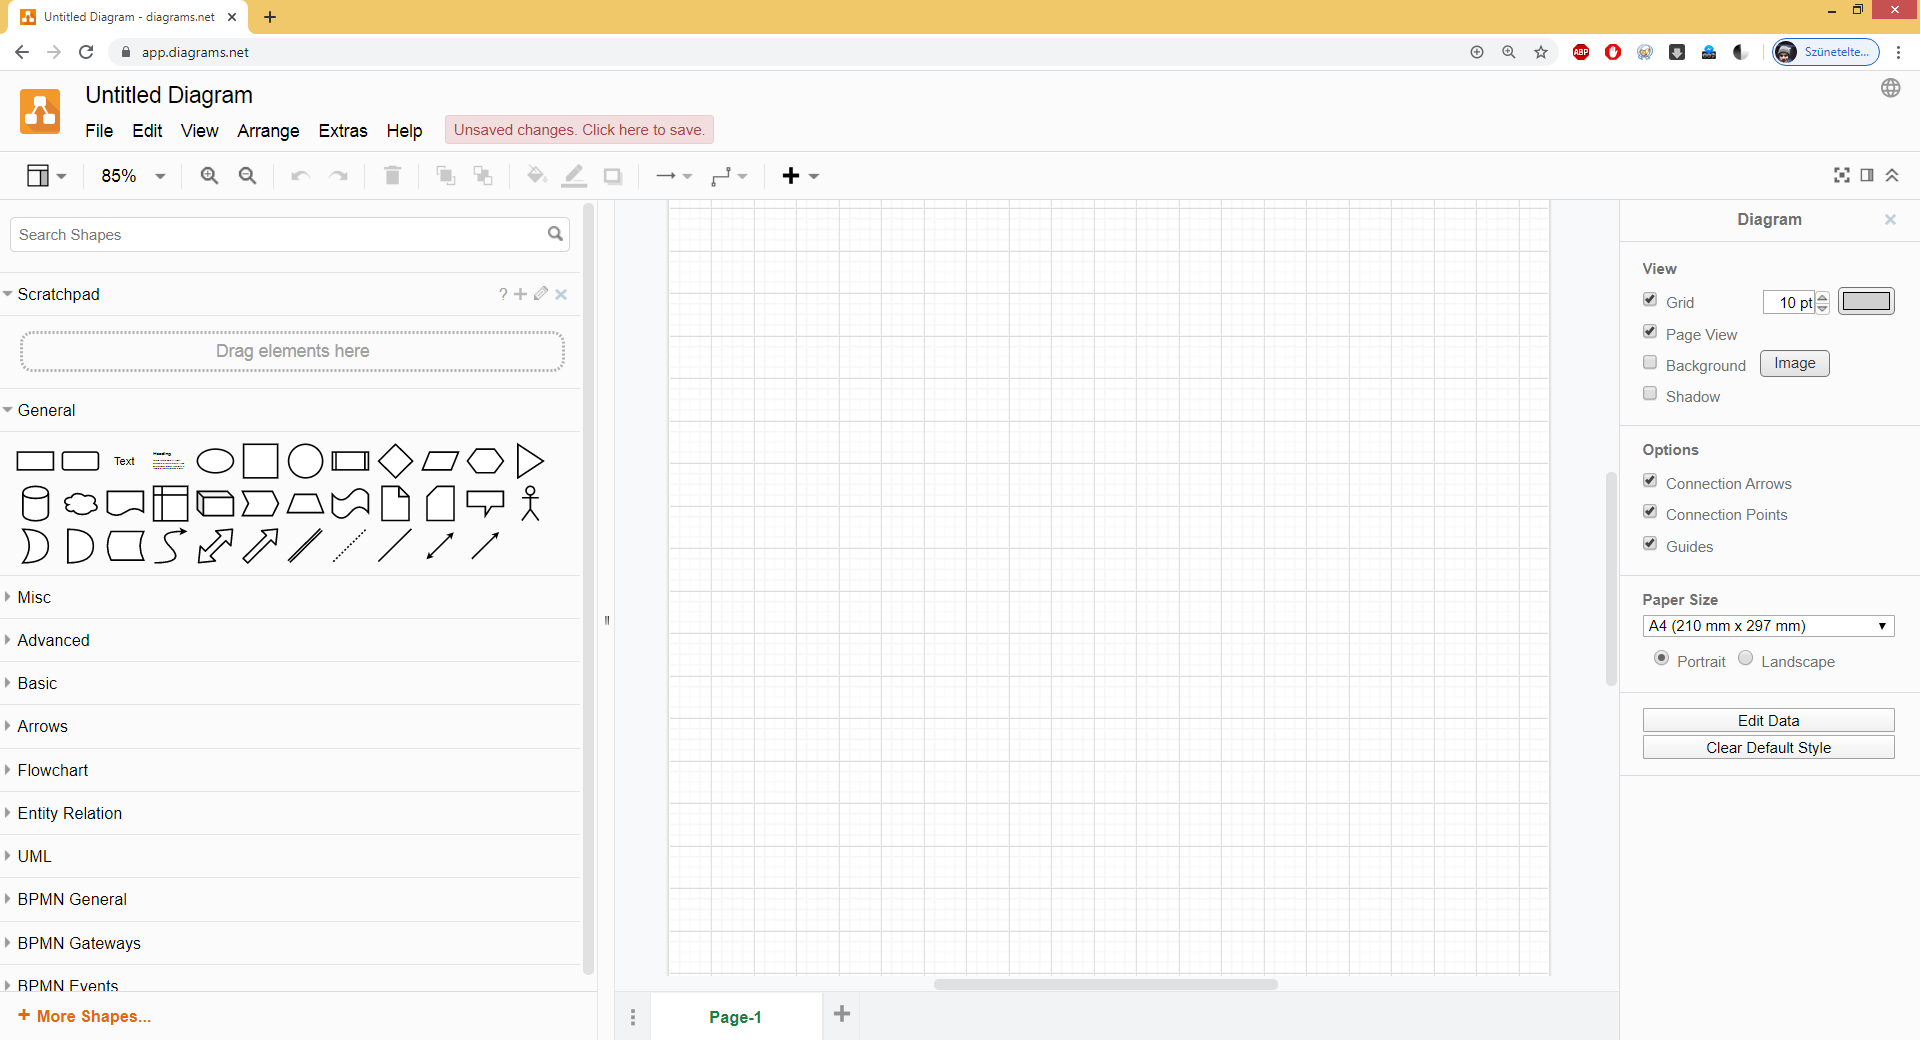
\includegraphics[scale=0.3]{images/drawio.png}
\caption{A Draw.io nyitóoldala (Forrás: draw.io)}
\label{fig:drawio}
\end{figure}

Láthatjuk, hogy rengeteg lehetőség tárul elénk. A modellezéshez nagyon sok féle szimbólum közül választhatunk számunkra megfelelőt. Termszetesen mindegyik más jelentéssel bír, azonban a program teljes egészében a felhasználóra bízza azok használatát: nem határoz meg integritási feltételeket, így a felhasználó szabályoktól függetlenül alakíthat ki számára kedvező ábrákat.

Használata viszonylag egyszerű, felhasználóbarát. A felhasználó kiválaszt egy elemet a bal oldali eszköztárból, és azt kattintással, vagy akár behúzással megjeleníti a képernyő közepén található négyzetrácsos részen. Az így megjelenített szimbólumokat nyomva tartott bal egérgomb mellett az egér mozgatásával lehet áthelyezni.

Az általános szimbólumokon kívül (amik a program bal oldali menüjében le vannak nyitva \textit{General} néven) különböző nyilakat, egyéb formákat használhatunk, UML diagramokat készíthetünk, illetve az üzleti folyamatmodell és jelölés (\textit{Business Process Model and Notation}, BPMN) sajátos alakzatait is igénybe vehetjük. De ha még ez se lenne elég, akkor lehetőség van az eszköztárat kibővíteni további alakzatok hozzáadásával, amit a bal alsó sarokban található \textbf{"More Shapes\ldots"} (további alakzatok) gomb megnyomásával.

Elkészített folyamatábráink / diagramjaink mentésére is többféle módot kínál az alkalmazás. Lehetőség van PNG, SVG, HTML, és XML formátumba is menteni a munkánkat, amiket a saját eszközünkre, vagy akár Google Drive-ra, GitHub-ra, és még sokféle felületre azonnal exportálhatunk is.

Összegezve tehát a Draw.io egy rendkívül hasznos és változatos alkalmazás, amely sokféle megvalósítási lehetőséget kínál a felhasználók számára. Egyszerű használatának köszönhetően népszerű a felhasználók körében. Üzleti folyamatok modellezésére kiválóan használható. Egyetlen hátránya lehet az, hogy (mivel böngészőből indítható el) internetkapcsolat szükséges hozzá, de ma már szinte bárhol vagyunk, könnyedén csatlakozni tudunk a világhálóhoz.

%\SubSection{Lucidchart}

%Második példaként bemutatható
